% Name: Arrows of each dimension
% Description: A 1-cell, a 2-cell, a 3-cell, and a 4-cell arrow, made of one to four strokes with the same spacing between them.
% Tags: nfold, higher category theory, n-cells, arrows

\usetikzlibrary{nfold, arrows.meta}

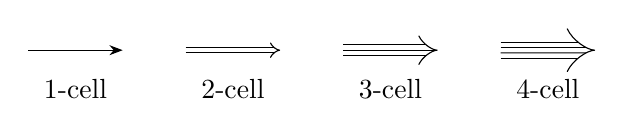
\begin{tikzpicture}[every node/.style={below=7pt}]
  \draw[-{Stealth}] (0,0) -- (1.2,0) node[midway] {$1$-cell};
  \draw[double equal sign distance, scaling nfold=2, arrows=-Implies] (2,0) -- (3.2,0) node[midway] {$2$-cell};
  \draw[double equal sign distance, scaling nfold=3, arrows=-Implies] (4,0) -- (5.2,0) node[midway] {$3$-cell};
  \draw[double equal sign distance, scaling nfold=4, arrows=-Implies] (6,0) -- (7.2,0) node[midway] {$4$-cell};
\end{tikzpicture}
